%!TEX root =  tfg.tex
\chapter{Etats des lieux}

\begin{quotation}[Novelist]{Ernest Hemingway (1899--1961)}
The good parts of a book may be only something a writer is lucky enough to overhear or it may be the wreck of his whole damn life -- and one is as good as the other.
\end{quotation}

\begin{abstract}
Resumen de lo que va a ocurrir en el capítulo. ¿Cuál es el objetivo que tenemos con este capítulo?
\end{abstract}

\section{Présentation de l'entreprise}
\subsection{Historique et localisation}
\subsubsection{Historique}
\begin{itemize}
    \item[*] Mazars dans le monde
    Mazars est une organisation internationale et indépendante, spécialisée dans l’audit, le conseil ainsi que les services comptables, fiscaux et juridiques. Au 1er janvier 2018, Mazars est présent dans les 86 pays et territoires qui forment son partnership international intégré. Mazars fédère les expertises de 20 000 femmes et hommes basés dans 300 bureaux à travers le monde. Emmenés par 960 associés, ils servent leurs clients à toutes les étapes de leur développement : de la PME aux grands groupes internationaux en passant par les entreprises intermédiaires, les start-ups et les organismes publics.
    
    Mazars est également membre fondateur de l’Alliance \textit{Praxity}, qui rassemble 66 organisations indépendantes et plus de 41 780 professionnels dans 103 pays.

    \item[*] Mazars au Cameroun
    En 2000, année 1 du 21e siècle, MAZARS, par son associé M. FANDOHAN a proposé à M. L. RIQUIER une intégration au partnership permettant ainsi à l’organisation de justifier d’une présence au Cameroun (Douala et Yaoundé) de 20 ans, d’un portefeuille clients en audit (50\%), en expertise comptable (20\%), et en conseil juridiques et fiscaux (20\%) de plus de 100 sociétés (OMB) dans les secteurs de l’industrie et des services dégageant un chiffre d’affaires de quatre cent millions de FCFA pour un effectif de 15 personnes.
    
    La Société Anonyme MAZARS Cameroun a été créée en 2002 agréée en CEMAC en 2005 et inscrite au tableau de l’ONECCA en 2006.
\end{itemize}
\subsubsection{Localisation}
Notre stage a été effectué à Bureau Mazars Cameroun situé à Douala, sis à l’Immeuble Ancien AMACAM. Mazars Cameroun a pour adresse : B.P. : 3791 Douala Cameroun, Tel : (+237) 233 42 42 47 – (+237) 233 42 55 48 – (+237) 233 42 41 14, Fax : (+237) 233 42 91 70, email : info@mazars.cm, site : www.mazars.cm.

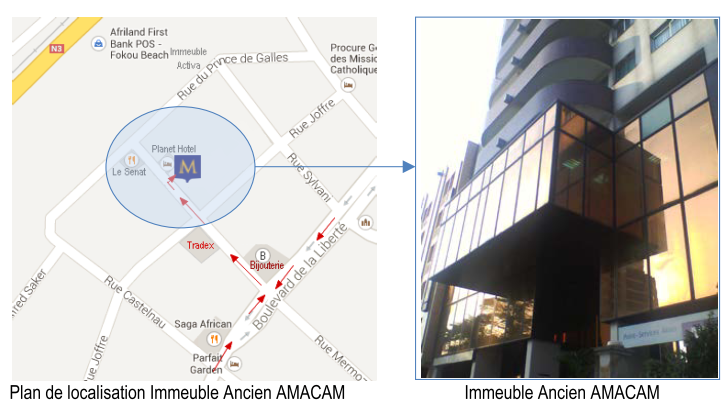
\includegraphics{localisation.png}

\subsection{Organisation générale de Mazars Cameroun}
Mazars Cameroun dispose de deux bureaux sur l’ensemble du territoire : 
\begin{itemize}
    \item Un bureau situé à Douala;
    \item Un second bureau situé à Yaoundé.
\end{itemize}
Notons que Mazars Cameroun est scnindé en deux principales unités:
\begin{itemize}
    \item Mazars Cameroun SA;
    \item Mazars TAX/LEGAL SA.
\end{itemize}
\begin{center}
    \begin{tabular}{c|c}
        \hline
         \textbf{Dénomination} & Mazars Cameroun SA  \\
         \textbf{Capital Social} & Vingt millions FCFA (20 000 000 FCFA) \\
         \textbf{Forme Juridique} & Société Anonyme (SA) \\
         \textbf{Boîte Postale} & 3791 Douala-Cameroun \\
         \textbf{Localisation} & Avenue Rue de Lapeyrere, Ancien Immeuble AMACAM, Douala \\
         \textbf{PDG} & M. Lucien Riquier \\
         \textbf{Logo} & 
\includegraphics{logo_M.png}
    \end{tabular}
\end{center}

\subsection{Secteur d'activité de Mazars Cameroun}
Mazars Cameroun est un cabinet d’expertise comptable qui fournit les lignes de service suivantes :
\begin{itemize}
    \item [-] Financial Audit
    \begin{itemize}
        \item[+] Audit légal
        \item[+] Audit contractuel
    \end{itemize}
    \item[-] Consulting
    \begin{itemize}
        \item[+] Gouvernance et maîtrise des risques
        \item[+] Stratégie et Opération
        \item[+] Développement durable
    \end{itemize}
    \item[-] Accounting and Outsourcing Services
    \begin{itemize}
        \item[+] Support fonction comptable et financière
        \item[+] Consolidation et \textit{Reporting}
        \item[+] Paie
        \item[+] Formalités fiscales
        \item[+] Sécrétariat juridique
    \end{itemize}
    \item[-] Financial Advisory Services
    \begin{itemize}
        \item[+] Litiges et fraudes
        \item[+] Financement de projet
        \item[+] \textit{Restructuring}
        \item[+] \textit{Transaction}
        \item[+] Modélisation et évaluation
    \end{itemize}
    \item[-] Tax Consulting
    \begin{itemize}
        \item[+] Fiscalité internationale-Douane
        \item[+] Fusion-Acquisition
        \item[+] Prix de transfert
    \end{itemize}
    \item[-]Legal Consulting
    \begin{itemize}
        \item[+] Droit des sociétés
        \item[+] Procédures collectives
        \item[+] Fusions et acquisitions
        \item[+] Banques et finances
        \item[+] Droit du travail
    \end{itemize}
\end{itemize}

\subsection{Présentation du département Consulting}
Notre stage s’est déroulé au sein du département consulting.  L’utilisation de plus en plus de l’outil informatique dans l’environnement de l’entreprise permet d’augmenter les chances d’atteindre leurs objectifs stratégiques. Toutefois, il faut associer à cela des dépenses substantielles dans le développement, l’implémentation et la maintenance de la technologie. 

Le département du Consulting a pour objectifs d’accompagner les clients à établir l’assurance que :
\begin{itemize}
    \item[-] \textbf{-	Les risques organisationnels clés sont correctement identifiés et évalués;}
    \item[-] \textbf{-	Les contrôles en place sont effectifs;}
    \item[-] \textbf{-	Les informations traitées sont conformes et sécurisées.}
\end{itemize}
Les Services offerts par ce département sont :
\begin{itemize}
    \item[-] \textbf{Audit}
    \begin{itemize}
        \item[+] Fonction informatique
        \item[+] Projets informatique
        \item[+] Exploitation
        \item[+] Applications opérationnelles
        \item[+] Sécurité informatique
    \end{itemize}
    \item[-] \textbf{Projects}
    \begin{itemize}
        \item[+] Diagnostic IT
        \item[+] Maturation des projets
        \item[+] Aide au choix de solutions IT
        \item[+] Mise en oeuvre
        \item[+] Conduite du changement
        \item[+] Accompagnement opérationnel
    \end{itemize}
    \item[-] \textbf{Sécurité de l'information}
    \begin{itemize}
        \item[+] Evaluation des vulnérabilités
        \item[+] Tests d'intrusion
        \item[+] Accompagnement ISO 270001
        \item[+] Revue Architecture de Sécurité
        \item[+] Analyse et Gestion de risques
        \item[+] Séminaire de formations
    \end{itemize}
\end{itemize}

\section{Etude de l'existant}
\subsection{Analyse Post-interviews}
Des interviews ont été réalisées au sein de chaque département de l'entreprise et les il est ressorti des ces interviews des éléments qui seront présentés dans la suite.
\subsubsection{Remarques}
Le département RH possède déjà un certain nombre de procédures rédigées. Cependant, ces procédures datent de 2013 et n’ont pas été mises à jour depuis cette date. Il convient donc de mettre à jour ces procédures afin de les aligner à la règlementation en vigueur. Les autres départements n’ont pas de procédures rédigées et validées.
\subsubsection{Actifs supports les plus sollicités au sein de l’entreprise}
\begin{itemize}
    \item[-] \textbf{Le serveur de messagerie:} qui permet d’échanger les mails au sein du cabinet mais aussi avec des entités externes;
    \item[-] \textbf{Le Serveur NAS :} : lieu de stockage de tous les documents numériques de l’entreprise : il s’agit en effet de la ressource la plus critique au sein de la structure et un niveau de protection adéquat doit être défini pour ce dernier ;
    \item[-] \textbf{Audisoft :} Il s’agit du logiciel utilisé dans le cadre des missions d’Audit. En communiquant avec son serveur GESTRAS il permet de mener à bien ces missions en stockant et en générant les fichiers nécessaires à l’accomplissement de la mission ;
    \item[-] \textbf{SAGE PAIE : }logiciel de gestion de la paie, il permet de gérer tous les paramètres liés à la paye des employés de Mazars mais aussi des clients ;
    \item[-] \textbf{SenatorFxLite : }logiciel de gestion des accès, gère les entrées et sorties au sein du cabinet ;
    \item[-] \textbf{PARRABELLUM : }logiciel de gestion des temps passés, permet de renseigner les temps passés sur une mission ou au sein du cabinet.
\end{itemize}
\subsubsection{Eléments redondants}
Nous avons remarqué que le processus d’archivage ne diffère pas vraiment d’un corps de métier à l’autre. En effet la seule différence remarquable se situe au niveau du temps de conservation après archivage ; mis à part ce détail, le processus reste le même.

\subsection{Etude comparative avec des solutions existantes}
La classification des données est essentielle pour les entreprises car elle permet de mieux protéger les informations détenues par l’entreprise. La classification des données permet aux utilisateurs d’attribuer une étiquette visuelle aux données qu’ils créent, de sorte que des décisions adéquates puissent être prises quant à leur manipulation (création, stockage, partage, suppression, etc.).

Les solutions de classification qui existent à l’heure actuelle consistent essentiellement en solutions logicielles. D’un autre côté, une autre approche consiste à adopter une démarche méthodologique afin d’aboutir à une politique de classification sur papier. Enfin une dernière approche consiste en une classification des données pilotée par l’utilisateur.[5]

\subsubsection{Utilisation d'un outil de classificaton automatisé}
La classification automatisée est basée sur un logiciel ou outil qui assiste l’utilisateur dans la classification réussie et précise de leurs fichiers de données. Cette classification peut être [6]:
\begin{itemize}
    \item[-] Entièrement automatisée;
    \item[-] Suggéré;
    \item[-] Prescite;
    \item[-] Approuvé par l'utilisateur.
\end{itemize}
Cette classification s’appuie en général sur des informations telles que l’emplacement de stockage des données, leur accessibilité, leur création et même leur contenu pour classer les données. Cette classification se fait généralement de la manière suivante :
\begin{itemize}
    \item[-] Ajout de métadonnées suivant le dossier dans lequel le document est stocké ;
    \item[-] Ajout de métadonnées suivant le lieu de stockage du document ;
    \item[-] Scan des documents afin d’identifier les sujets et thèmes desquels une classification sera suggérée ;
    \item[-] Ajout d’éléments visuels de marquage (en tête, pied de page, filigrane).
\end{itemize}

\textbf{Avantages d'une solution automatisée}
\begin{itemize}
    \item[-] Rapide retour sur Investissement car les résultats seront produits dans des délais assez courts ;
    \item[-] Réduction des erreurs humaines ;
    \item[-] Pas besoin d’une large communication ni de programmes de formation.
\end{itemize}

\textbf{Inconvénients d'une solution automatisée}
\begin{itemize}
    \item[-] Incompréhension du contexte de travail ce qui peut engendrer des sorties inexactes ;
    \item[-] Production de faux positifs qui peuvent entraver les processus métiers ;
    \item[-] Production de faux négatifs qui peuvent entraîner une perte de données.
\end{itemize}

\subsubsection{Classification des données par l'utilisateur}
Ici, les employés sont responsables de décider quelle étiquette est appropriée pour une information ; cet attachement se fait à travers un logiciel au moment de la création, envoi, modification ou enregistrement du fichier.
\textbf{Avantages}
\begin{itemize}
    \item[-] L’utilisateur est plus impliqué dans le contexte ce qui lui permet de définir correctement l’étiquette à appliquer à une donnée ;
    \item[-] Il s’agit d’une couche de sécurité supplémentaire utilisée souvent pour compléter la classification automatisée.
\end{itemize}
L'inconvénient de cette approche est qu'elle prend du temps pour être mise en place. Les employés doivent être formés afin de connaître exactement quelle étiquette associer à une information.

\subsubsection{Politique de classification sur papier}
Il s’agit ici d’élaborer une politique de classification que chaque employé manipulant des informations devra utiliser afin d’étiqueter celles-ci. Dans cette approche l’on doit s’assurer que les employés s’alignent à cette politique et à la politique globale de sécurité de l’entreprise. Une politique bien définie permet aux employés de prendre rapidement des décisions intuitives quant à l’étiquette à fournir à une donnée. 

L’inconvénient avec cette approche qui n’a aucun soutien technologique est qu’il faut mettre en place des contrôles pour s’assurer que tout le monde est au courant de la politique et la met en place. 

Le tableau de comparaison ressort les différences et corrélations entre les solutions de classification existantes suivants un ensemble de critères bien définis.
\begin{center}
    \begin{tabular}{c|c|c|c}
        \hline
         \textbf{Critère de comparaison} & \textbf{Classification automatisée} & \textbf{Classification dirigée par l'utilisateur} & \textbf{Classification sur papier}  \\
        \hline
         Rapidité des résultats fournis & Grande & Moyenne & Faible \\
         \hline
         Fiabilité des résultats & Moyenne & Grande & Moyenne \\
         \hline
         Réduction des erreurs humaines & Grande & Grande & Faible \\
         \hline
         Compréhension du contexte de travail & Faible & Moyenne & Grande \\
         \hline
         Taux de faux positifs & Grand & Faible & Faible \\
         \hline
         Taux de faux négatifs & Grand & Faible & Faible \\
         \hline
         
    \end{tabular}
\end{center}